\chapter{Statistical Power}
\section{Statistical Power}
\begin{definition}[Power of a Test]
The probability that a fixed level $\alpha$ significance test will reject $H_0$ when a particular alternative value of the parameter is true is called the \textbf{power} of the test against that alternative.
\end{definition}

The statistical power of a test is its ability to detect an effect if it exists in reality.

It is the probability of correctly rejecting $H_0$ when $H_0$ is false in reality.

\begin{equation*}
\text{Power} = P(\text{reject } H_0 \mid H_0 \text{ false})
\end{equation*}

\begin{equation*}
0 < \text{power} < 1
\end{equation*}

Power close to 1 (high power):\\
\quad Test is good at detecting effects.\\

Power close to 0 (low power):\\
\quad Test is not reliable (i.e., we expect the test will not reject $H_0$ when $H_0$ is false).

\vspace{1em}
Power is affected by:

\begin{itemize}
 \item \textbf{The effect} \\ (\textcolor{blue}{larger differences between reality and the null are easier to detect})

  \item \textbf{Sample size} \\ (\textcolor{blue}{larger samples increase power})

  \item \textbf{Significance level} ($\alpha$) \\ (\textcolor{blue}{as $\alpha$ increases, easier to reject $H_0$})

  \item \textbf{Variability in data} \\ (\textcolor{blue}{lower variability, higher power})
\end{itemize}
\subsection*{Type I and II Errors}

It is possible to make an incorrect conclusion on a hypothesis test. \\

\textbf{Type I:} Incorrectly reject $H_0$ when $H_0$ is true in reality. \\
\textbf{Type II:} Incorrectly fail to reject $H_0$ when $H_0$ is false in reality. \\


\noindent \textbf{Reality vs Conclusion Table:}
\vspace{1em}
\begin{center}
\small
\renewcommand{\arraystretch}{1.8}
\setlength{\tabcolsep}{1.5em}

\text{Reality}

\vspace{0.5em}

\begin{tabular}{c c}
\hspace*{2em}\rotatebox[origin=c]{90}{\textbf{Conclusion}} &
\begin{tabular}{|l|c|c|}
\hline
& $H_0$ True & $H_0$ False \\
\hline
\textbf{Reject $H_0$} & \textcolor{red}{Type I ($\alpha$)} & \textcolor{green!50!black}{No error \checkmark} \\
\hline
\textbf{Fail to reject $H_0$} & \textcolor{green!50!black}{No error \checkmark} & \textcolor{red}{Type II ($\beta$)} \\
\hline
\end{tabular}
\end{tabular}
\end{center}



\vspace{1em}
\textbf{\textit{Note:}} Type I errors are generally considered worse.

\vspace{0.5em}
\noindent Let $\beta$ be the probability of a Type II error. Then:

\[
\text{Power} = 1 - \beta = 1 - P(\text{Type II})
\]
\begin{example}[Sweetening Colas: Power]
The cola maker determines that a sweetness loss is too large to accept if the mean response for all tasters is $\mu = 1.1$. Will a 5\% significance test detect this?

\textbf{Hypotheses:}
\[
\begin{aligned}
H_0\!:&\ \mu = 0 \\
H_A\!:&\ \mu > 0
\end{aligned}
\]

Assume:
\[
n = 10, \quad \sigma = 1, \quad \alpha = 0.05
\]

\textbf{Step 1: Determine the rejection region.}

Since the test is one-sided with $\alpha = 0.05$, we find:
\[
z_{\text{crit}} = 1.645 \quad \text{(from Z-table)}
\]

We reject $H_0$ if:
\[
Z^* > 1.645
\]

\begin{center}
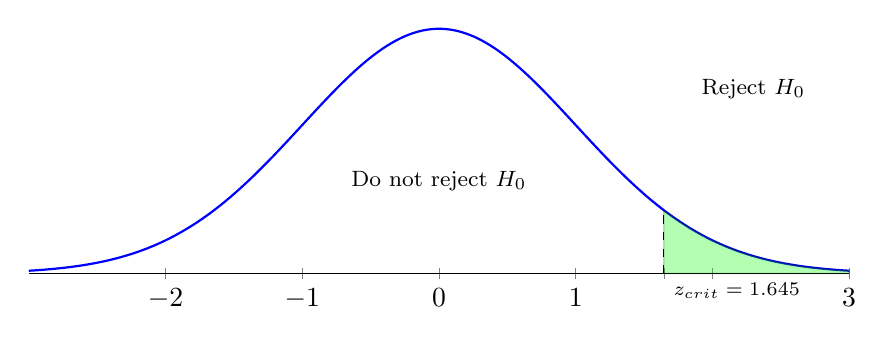
\begin{tikzpicture}
\begin{axis}[
  domain=-3:3,
  samples=200,
  xlabel={},
  ylabel={},
  ymin=0,
  xtick={-2,-1,0,1,1.645,2,3},
  xticklabels={$-2$,$-1$,$0$,$1$,,,$3$},
  ytick=\empty,
  width=12cm,
  height=5cm,
  clip=false,
  axis x line=bottom,
  axis y line=none,
  axis line style={-}, % ensures it's a regular solid line
]

% Standard normal curve
\addplot[blue, thick, no markers, domain=-3:3, samples=200] {exp(-x^2/2)/sqrt(2*pi)};

% Rejection region
\addplot[domain=1.645:3, fill=green, opacity=0.3] {exp(-x^2/2)/sqrt(2*pi)} \closedcycle;

% Critical line
\draw[dashed] (axis cs:1.645,0) -- (axis cs:1.645,{exp(-1.645^2/2)/sqrt(2*pi)});
\node[below right] at (axis cs:1.645,0) {\scriptsize $z_{\text{crit}} = 1.645$};

% Add regions
\node at (axis cs:0, 0.15) {\footnotesize Do not reject $H_0$};
\node at (axis cs:2.3, 0.3) {\footnotesize Reject $H_0$};


\end{axis}
\end{tikzpicture}
\vspace{0.5em}
\captionof{figure}{Rejection region for $Z$ with $\alpha = 0.05$}
\end{center}


\textbf{Step 2: Find the equivalent critical value of } $\bar{x}$.

Since $\sigma$ is known,
\[
Z = \frac{\bar{x} - \mu_0}{\sigma/\sqrt{n}} \quad \Rightarrow \quad
1.645 = \frac{\bar{x}_{\text{crit}} - 0}{1/\sqrt{10}} \Rightarrow \bar{x}_{\text{crit}} \approx 0.520
\]

So we reject $H_0$ if $\bar{x} > 0.520$.

\textbf{Step 3: Calculate the power when $\mu = 1.1$ is true.}

\[
P\left(Z > \frac{0.520 - 1.1}{1/\sqrt{10}}\right)
\approx P(Z > -1.83) = 1 - 0.0336 = 0.9664
\]


\textbf{Interpretation:} There is a 96.6\% chance the test correctly detects $\mu = 1.1$.

\vspace{1em}

\begin{center}
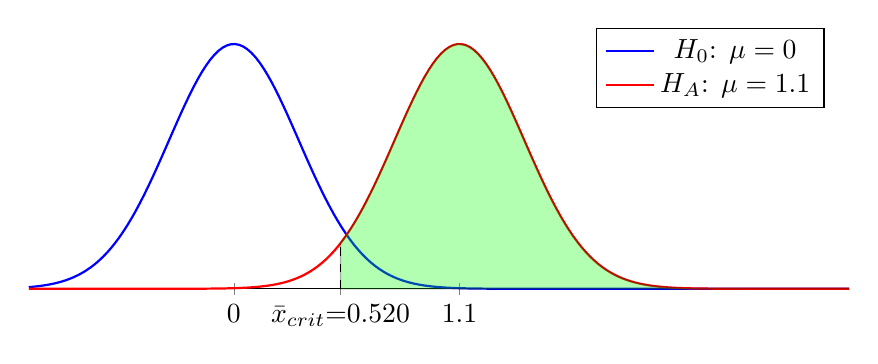
\begin{tikzpicture}
\begin{axis}[
  domain=-1:3,
  samples=200,
  xlabel={},
  ylabel={},
  ymin=0,
  xtick={0,0.52,1.1},
  xticklabels={$0$, $\bar{x}_{\text{crit}}{=}0.520$, $1.1$},
  ytick=\empty,
  width=12cm,
  height=5cm,
  clip=false,
  axis x line=bottom,
  axis y line=none,
  axis line style={-}, % ensures it's a regular solid line
  legend style={at={(0.97,0.97)}, anchor=north east},
]

% H0 distribution (mean = 0)
\addplot[blue, thick] {exp(-(x)^2/(2 * (1/sqrt(10))^2)) / (sqrt(2*pi) * (1/sqrt(10)))};
\addlegendentry{$H_0$: $\mu = 0$}

% HA distribution (mean = 1.1)
\addplot[red, thick] {exp(-(x - 1.1)^2/(2 * (1/sqrt(10))^2)) / (sqrt(2*pi) * (1/sqrt(10)))};
\addlegendentry{$H_A$: $\mu = 1.1$}

% Shade rejection region under H_A
\addplot[domain=0.52:3, fill=green, opacity=0.3] 
  {exp(-(x - 1.1)^2/(2 * (1/sqrt(10))^2)) / (sqrt(2*pi) * (1/sqrt(10)))} 
  \closedcycle;

% Dashed line for x_crit
\draw[dashed] (axis cs:0.52,0) -- (axis cs:0.52, {exp(-(0.52 - 1.1)^2/(2 * (1/sqrt(10))^2)) / (sqrt(2*pi) * (1/sqrt(10)))});
\end{axis}
\end{tikzpicture}
\vspace{0.5em}
\captionof{figure}{Power curve showing shaded rejection area under $H_A$}
\end{center}

\end{example}
\section{Type I and Type II Errors}

If we reject $H_0$ when in fact $H_0$ is true, this is a \textbf{Type I error.} \\

If we fail to reject $H_0$ when in fact $H_a$ is true, this is a \textbf{Type II error.} \\

The \textbf{significance level} $\alpha$ of any fixed level test is the probability of a Type I error. \\

The \textbf{power} of a test against any alternative is 1 minus the probability of a Type II error for that alternative. \\

The probability of making a Type II error is denoted by $\beta$. 
\begin{tcolorbox}[title=\textbf{Decision Errors in Tests},
  colback=yellow!10,
  colframe=black!45,
  coltitle=black,
  fonttitle=\bfseries,
  breakable]

\textbf{Type I Error} \\
$H_0$ is true, but sampling variation in the data leads you to reject $H_0$, you’ve made a Type I error. \\
When $H_0$ is true, a Type I error occurs if $H_0$ is rejected. \\

\textbf{Type II Error} \\
$H_0$ is false, but sampling variation in the data does not lead you to reject $H_0$, you’ve made a Type II error. \\
When $H_0$ is false, a Type II error occurs if $H_0$ is \textbf{NOT} rejected.

\end{tcolorbox}

\begin{example}
According to Access and Support to Education and Training Survey (2008), of 4,756 adult Canadians, 1,581 indicated that they worked at a job or business at anytime (between July 2007 and June 2008), regardless of the number of hours per week.

Is there evidence to suggest that the true proportion $p$ is greater than 0.50?

\begin{align*}
H_0\!:&\ p = 0.50 \\
H_a\!:&\ p > 0.50
\end{align*}


\noindent\textbf{R Output}
\begin{tcolorbox}[colback=gray!10, colframe=black!45, arc=2mm]
\begin{verbatim}
prop.test(x = 1581, n = 4756, p = 0.50,
          alternative = "greater", correct = FALSE)

## 
##  1-sample proportions test without continuity
##  correction
## 
## data:  1581 out of 4756, null probability 0.5
## X-squared = 534.24, df = 1, p-value = 1
## alternative hypothesis: true p is greater than 0.5
## 95 percent confidence interval:
##  0.3212845 1.0000000
## sample estimates:
##         p 
## 0.3324222 
\end{verbatim}
\end{tcolorbox}


\textbf{$P\text{-value} > \alpha = 0.05$}; we Fail to Reject $H_0$.

\textbf{This means we could be making a Type II error.}We indicated that there is no evidence to conclude that the true proportion of adult Canadians who worked at a job or business at anytime (between July 2007 and June 2008), regardless of the number of hours per week, was more than 0.50 — this conclusion implies that $H_0: p = 0.50$ is plausible, but we could be wrong.
\begin{figure}[H]  % Use [H] to prevent floating (requires \usepackage{float})
\centering
\includegraphics[width=0.75\textwidth]{section13/images/power_curve.pdf}
\caption{\textit{Power curve for a one-sided test with points at $\mu = 0.52$ and $\mu = 1.1$}}
\end{figure}

\end{example}
\begin{example}[Cola Bottles: Power Analysis]


Bottles of a popular cola are supposed to contain 300 milliliters (ml) of cola. There is some variation from bottle to bottle because the filling machinery is not perfectly precise. The distribution of contents is Normal with standard deviation $\sigma = 3$ ml. Will inspecting 6 bottles discover underfilling?

The hypotheses are:
\begin{align*}
H_0\!:&\ \mu = 300 \\
H_a\!:&\ \mu < 300
\end{align*}

A 5\% significance test rejects $H_0$ if $z_* \leq -1.645$, where the test statistic $z_*$ is:
\[
z_* = \frac{\bar{x} - 300}{3 / \sqrt{6}}
\]

Power calculations help us see how large a shortfall in the bottle contents the test can be expected to detect. Find the power of this test against the alternative $\mu = 299$.

\vspace{1em}
\textbf{Step 1. Write the rule for rejecting $H_0$ in terms of $\bar{x}$.}

We know that $\sigma = 3$, so the $z$ test rejects $H_0$ at the $\alpha = 0.05$ level when:
\[
z = \frac{\bar{x} - 300}{3 / \sqrt{6}} < -1.645
\]

This is the same as:
\[
\bar{x} < 300 - 1.645 \cdot \frac{3}{\sqrt{6}} \quad \Rightarrow \quad \bar{x} < 297.985
\]

\vspace{1em}
\textbf{Step 2. The power is the probability of this event under the condition that the alternative $\mu = 299$ is true.}

To calculate this probability, standardize $\bar{x}$ using $\mu = 299$:
\[
\begin{aligned}
\text{power} &= P(\bar{x} < 297.985 \mid \mu = 299) \\
&= P\left( Z < \frac{297.985 - 299}{3 / \sqrt{6}} \right) \\
&= P(Z < -0.83) = 0.2033
\end{aligned}
\]

\end{example}
\section{Using Power to Determine Sample Size}




